\documentclass{article}

\usepackage{notes}
\usepackage{array}
\usepackage{amsmath}
\usepackage{mathtools}
\usepackage{graphicx}
\usepackage{amssymb}
\usepackage[a4paper,margin=0.5in]{geometry}

\graphicspath{{./Images/}}

\everymath{\displaystyle}
\DeclarePairedDelimiter{\ceil}{\lceil}{\rceil}

\begin{document}

\title{IVR Condensed Summary Notes For Quick In-Exam Strategic Fact Deployment }
\author{Maksymilian Mozolewski}
\maketitle


\pagebreak
\nSection{Introduction to Vision}

\nDefinition{Computer vision}{Processing data from any modality which uses the electromagnetic spectrum and produces an image}
\nDefinition{Image}{Way of representing data in a picture-like format, with a direct correspondence to the scene being imaged}
\nDefinition{CCD Camera}{
    Charged couple device, light falls on an array of MOS capacitors (which are rectangular and not square). The capacitors form a shift register and output either a line at a time or the whole array at one time (line vs frame transfer)
    
    \centering
    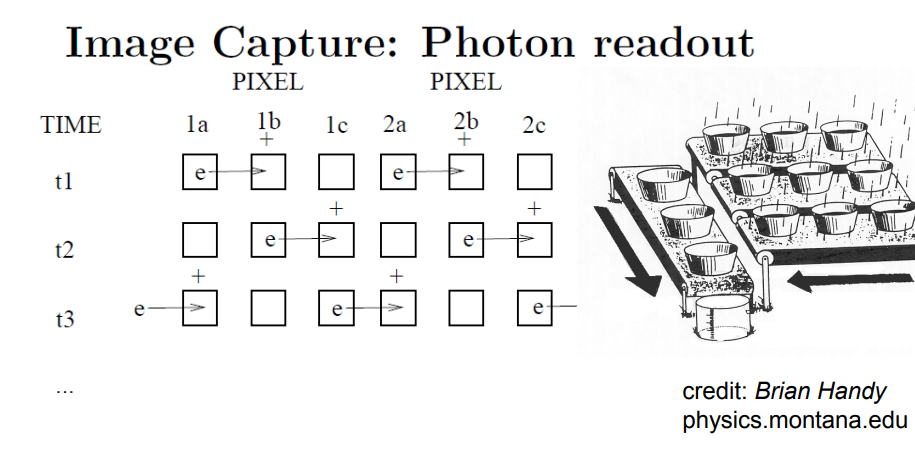
\includegraphics[width=0.5\columnwidth]{ccd_camera.png}

    \raggedright
    these "buckets" can overflow, resulting in over-saturation of the image
    }
\nDefinition{Frame grabber}{Device which converts analog image signals to digital image signals. Essentially puts a discrete value on each pixel signal. 24bit color is usually required for robotics}
\nDefinition{Visual Erosion}{RGB is a function of the sensitivity of the sensor to reflected light of each color. The sum of those intensities may vary wildly from frame to frame depending on the distance of the object due to intensity of the reflected light. The object appears to "errode" with changes in lighting. CCD Cameras are also notoriously insensitive to red, meaning that one of the three color planes is not as helpful in distinguishing colors. HSI and SCT colour spaces aim to reduce visual erosion since the Hue - the main wavelength measured (\textbf{perceptually meaningful dimensions}) will not change with the object's relative position, only its saturation and intensity will! Equipment to capture HSI images is expensive, and conversions between colour spaces sometimes fail.}
\nDefinition{Region Segmentation}{Finding groups of pixels related to each other via color, within a certain threshold and identifying the centroids of those groups. Requires high contrast between the \textbf{foreground} (object of interest) and the \textbf{background} to work well.}

\nDefinition{Color histogramming}{
    a type of histogram (bar chart basically), the user specifies range of values for each bar, 
    (bucket) the size of the bar is the number of data points falling within the bar's "range". 
    These ranges could be set to capture different values of either the R,G,B color intensities.

    \centering
    \includegraphics[width=0.7\columnwidth]{"histogram.png"}

    \raggedright
    Such histograms can be \textbf{subtracted bucket-wise} from each other as a form of distance measure to compare image stimuli.
}

\nDefinition{Stereopsis}{The method of triangulating depth data from 2 POV's}
\nDefinition{Stereo camera pairs}{Usage of two cameras to extract range data by finding the same point on the images received from two (most likely parallel) cameras, and then finding the depth information using the geometry of the cameras. It can be hard to find the same point on two pictures ()\textbf{correspondence problem}), the method of picking a spot of interest is called an \textbf{interest operator}. Cameras can be mounted in parallel to produce \textbf{rectified images} (the distance between the two cameras is then known as the \textbf{disparity}). This can save computation time since the point of interest will appear in the same line of the image on both cameras (\textbf{epipolar lines})}

\nDefinition{Optic flow}{Information to do with: Shadow cues, texture, expected size of objects}
\nDefinition{Light stripping}{
    Method of projecting a pattern of light onto a surface of interest and observing the distortion to the pattern to visualise the surface and/or distance information. Does not work that well in natural conditions due to noise.
    
    \centering 
    \includegraphics[width=0.4\columnwidth]{"light_stripper.png"}
    
}

\nDefinition{Laser ranging}{like radar but using light (\textbf{lidar}), scanning components are expensive, a planar laser range finder is a cheaper alternative. Produces an intensity and range map.}
\nDefinition{Range segmentation}{Segmenting the image based on range data, can be used to determine the geometry of surfaces}

\nSection{Image Basics}


\nTheorem{Homogenous coordinates}{
    Homogenous (aka similar) coordinates are coordinates in space with one more dimension than in the corresponding cartesian space, in this space we can express linear translations as linear matrix transformations!
    Every point in the cartesian space becomes a line in the homogenous space!

    \centering
    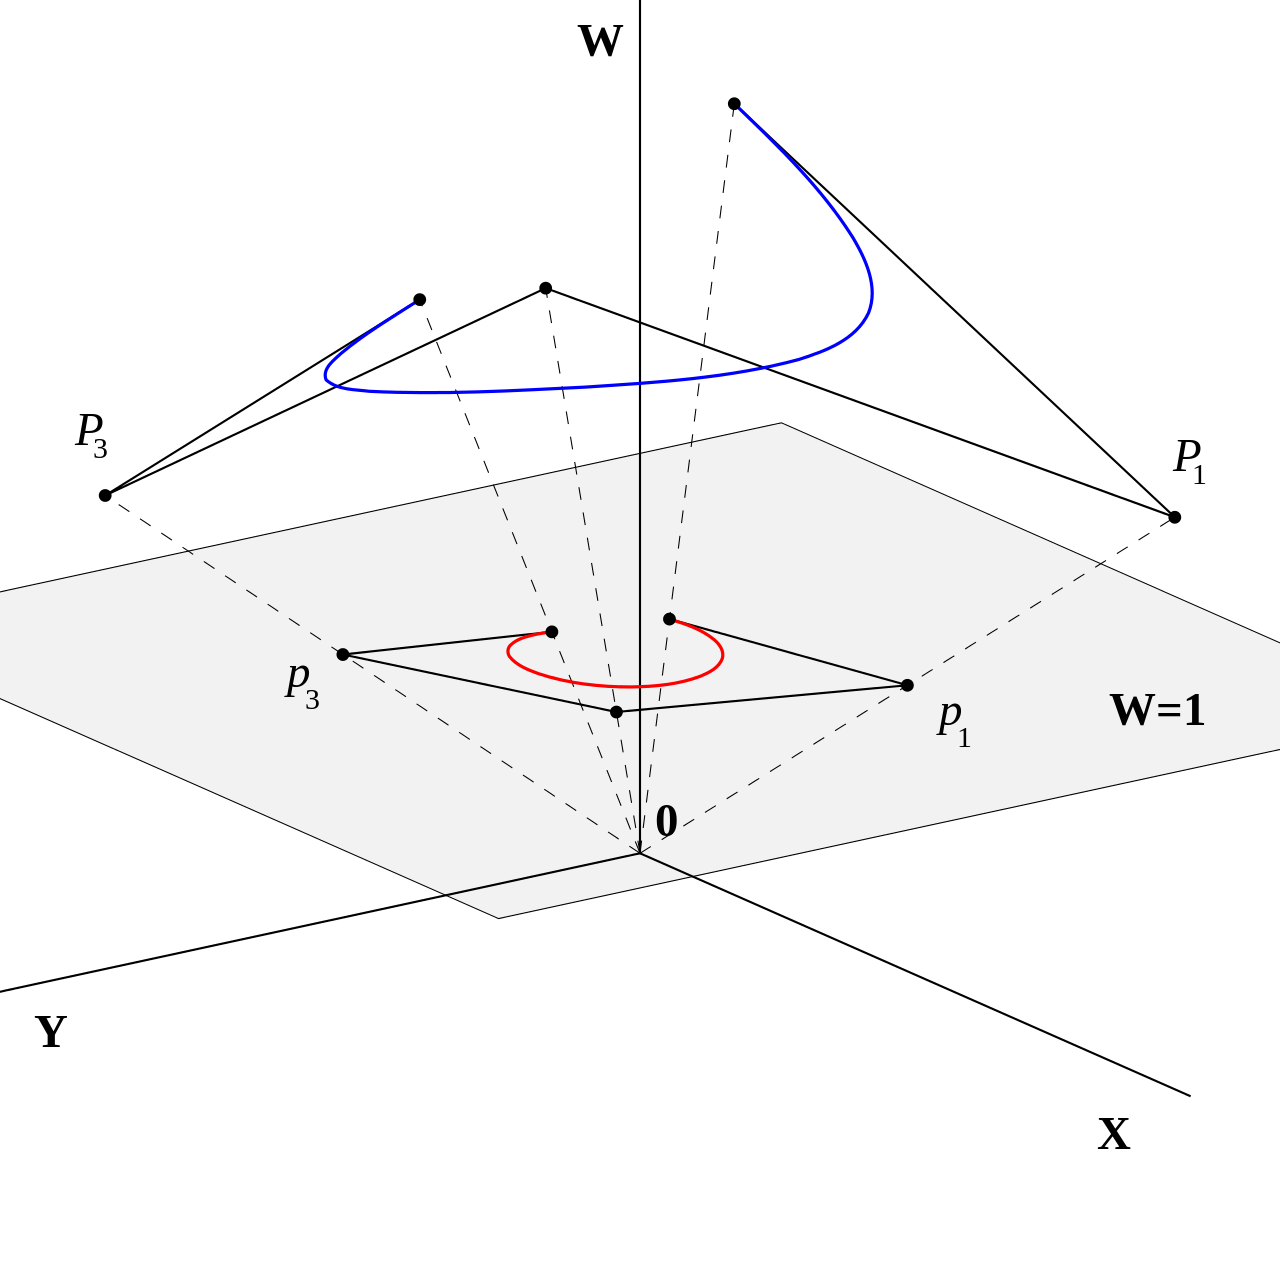
\includegraphics[width=0.5\columnwidth]{homogenous.png}

    \raggedright
    Conversion to homogenous coordinates:
    \begin{equation}
        \begin{bmatrix}
            x \\ y \\ \vdots \\  
        \end{bmatrix}
        = 
        \begin{bmatrix}
            x \\ y \\ \vdots \\ 1
        \end{bmatrix}
    \end{equation}

    Conversion from homogenous coordinates
    \begin{equation}
        \begin{bmatrix}
            x \\ y \\ \vdots \\ w
        \end{bmatrix}
        = 
        \begin{bmatrix}
            x/w \\ y/w \\ \vdots
        \end{bmatrix} 
        \quad w \neq 0
    \end{equation}

    Notice how a point in homogenous space can be multiplied by any constant, and yet when it is converted back to normal space, it becomes the same point. \textbf{The ratio} between the components defines the line in homogenous space.
}

\nDefinition{Pinhole camera}{
    
    Capturing on a simple plane does not work because multiple rays from the same point in the scene travel to multiple parts of the film. We want the film to capture a single "ray" per point of interest
    \begin{center}
    \begin{tabular*}{\columnwidth}{m{0.5\columnwidth}m{0.5\columnwidth}}
        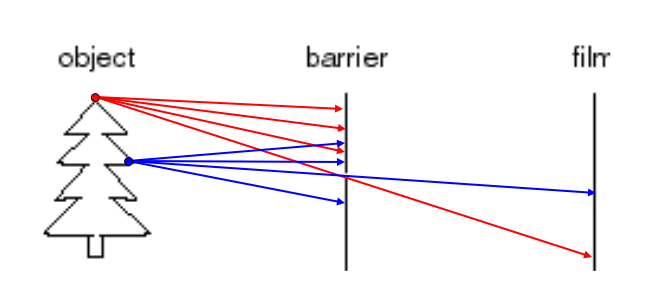
\includegraphics[width=0.45\columnwidth]{pinhole_failure.png}&
        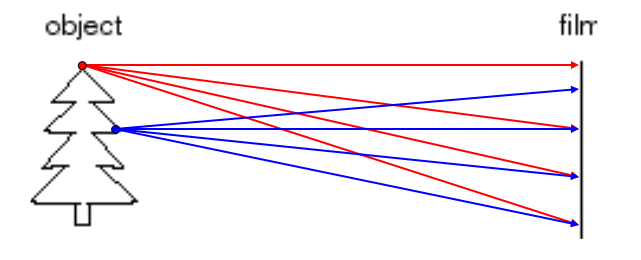
\includegraphics[width=0.45\columnwidth]{pinhole_failure_2.png}
    \end{tabular*}
    \end{center}

    A camera setup using a tiny hole to filter and hence focus the light onto a single clear image.

    \centering 
    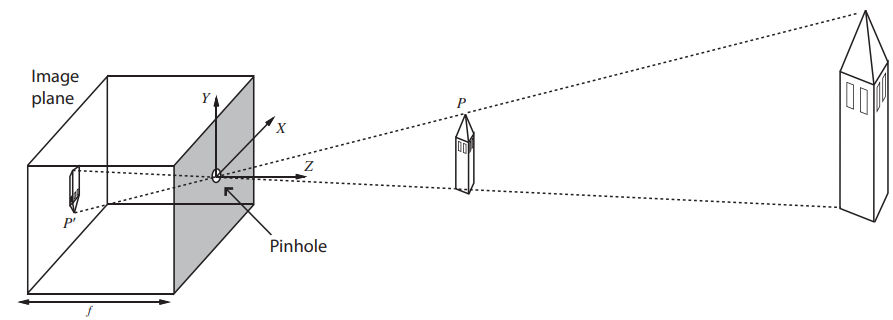
\includegraphics[width=0.6\columnwidth]{pinhole.png}
    
    \raggedright
    Using similar triangles, the point P:$(X,Y,Z)$ maps to point P' on the 2d surface of the image plane, at a distance f (\textbf{focal length}) from the pinhole as follows: 
    \begin{equation}
        x = \frac{-fX}{Z},
        y = \frac{-fY}{Z},
        z = f
    \end{equation}

    This projection of scene point to camera point can be expressed as a linear matrix transformation in homogenous space:

    \begin{equation}
        P_{h} =
        \begin{bmatrix}
            X \\ Y \\ -Z/f
        \end{bmatrix}
        =
        \begin{bmatrix}
            1 & 0 & 0 & 0 \\
            0 & 1 & 0 & 0 \\
            0 & 0 & -1/f & 0 
        \end{bmatrix}
        \begin{bmatrix}
            X \\ Y \\ Z \\ 1
        \end{bmatrix}
    \end{equation}

    To retrieve the projected point in cartesian space we simply divide by the third coordinate and discard it.

    \begin{equation}
        P_{c} = 
        \begin{bmatrix}
            X / (-Z/f) \\ Y / (-Z/f)
        \end{bmatrix}
        = 
        \begin{bmatrix}
            -fX/Z \\ -fY/Z
        \end{bmatrix}
    \end{equation}
    Which is identical to the projection above.

    This projection, preserves straight lines (\textbf{colinearity}) and their intersections, but looses information about angles and lengths (due to multiple points in 3D possibly mapping to the same point in 2D)
    
    Lines directly passing through the focal point are projected as points.
    
    Planes are preserved but those passing through the focal point are projected as lines.
}


\nTheorem{Vanishing point}{
    Any two parallel lines will converge to a certain point on the image as long as their directions are the same
    
    \begin{center}
    \begin{tabular*}{\columnwidth}{m{0.5\columnwidth}m{0.5\columnwidth}}
        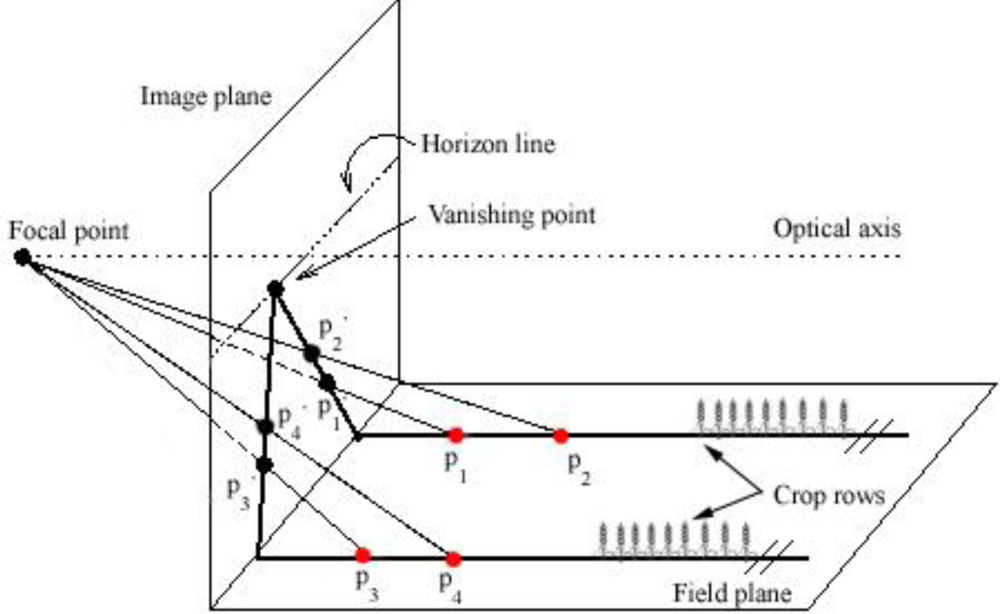
\includegraphics[width=0.45\columnwidth]{vanishing_point.png}&
        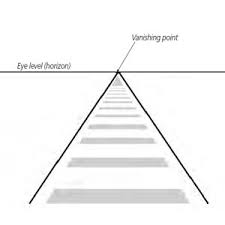
\includegraphics[width=0.45\columnwidth]{vanishing_road.jpeg}
    \end{tabular*}
    \end{center}
}

\nDefinition{Detector response curve}{
    The curve showing which frequencies of light a detector perceives the most and which will dominate the actual "perceived" or "central" wavelength of light, 
    i.e. the curve showing which wavelength of light a detector is most sensitive to.
    Each sensor type acts as a filter to the incomming light, and can produce an output signal proportional to the amount of its central wavelength absorbed.
    \\
    \par
    The wavelength signal perceived is a function of many things:
    \begin{itemize}
        \item type of source light
        \item the reflective properties of the objects in the scene 
        \item the sensor detector curve
    \end{itemize}

    As such knowing the "real" wavelength of the light is very difficult.
    
    \begin{center}
    \begin{tabular*}{\columnwidth}{m{0.5\columnwidth}m{0.5\columnwidth}}
        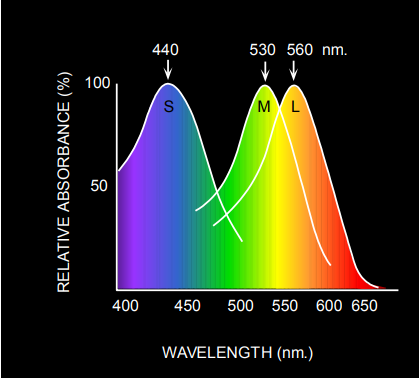
\includegraphics[width=0.45\columnwidth]{sensor_curves.png}&
        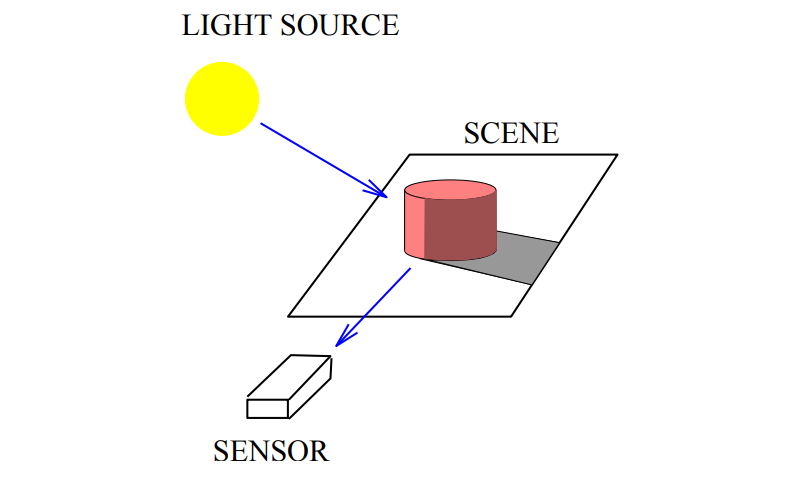
\includegraphics[width=0.45\columnwidth]{sensor_function.png}
    \end{tabular*}
    \end{center}
}

\nSection{Problems with image capture}

\nDefinition{Focus problems}{
    Focus set to one distance, and other nearby distances in focus (depth of focus). Further or closer not so well focused.
    
    \centering
    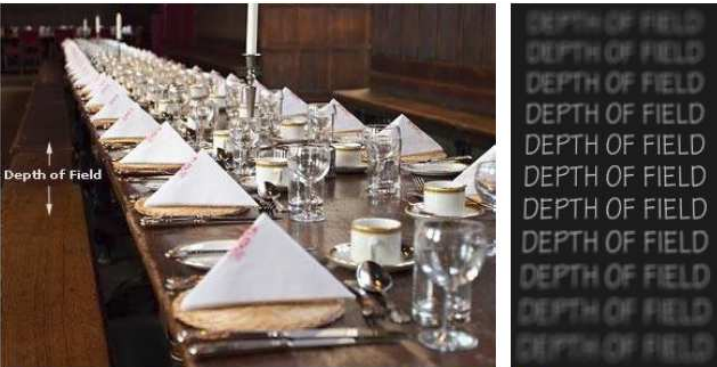
\includegraphics[width=0.3\columnwidth]{focus_problem.png}
    
    \raggedright
    Solutions: Use smaller aperture and brighter light
}

\nDefinition{Shadow problems}{
    False colours due to different intensity of light (shadows) make it difficult to separate shapes of interest from shadows.
    (is the white part under this part a shadow or the edge ?)

    Main cause of problem: point of light sources, the perceived brightness at a surface is proportional to the \textbf{square} of the distance between the surface and the light source.

    \centering
    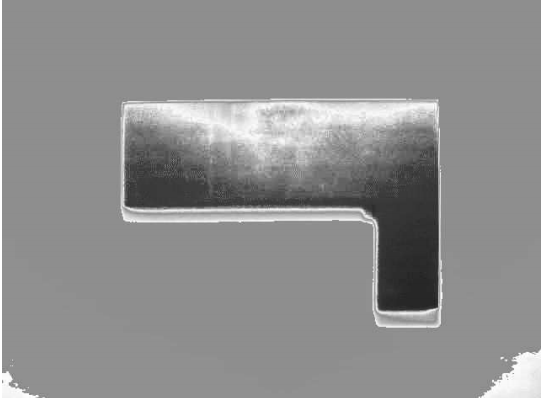
\includegraphics[width=0.3\columnwidth]{shadow_problems.png}
    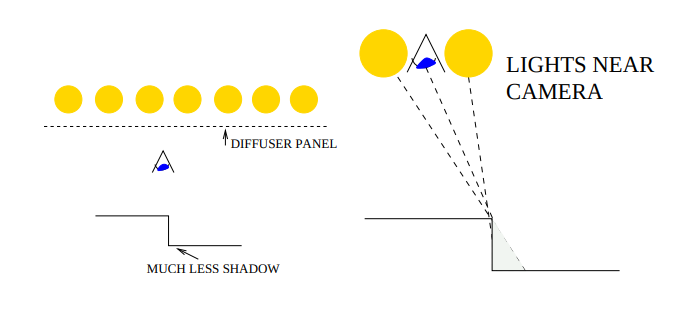
\includegraphics[width=0.6\columnwidth]{diffuser_panels.png}

    \raggedright
    Solutions: increase ambient lighting by using diffusing panels or lots of point lights
    }

\nDefinition{Specularities/highlights}{
    (Saturated pixels set to red)

    \centering
    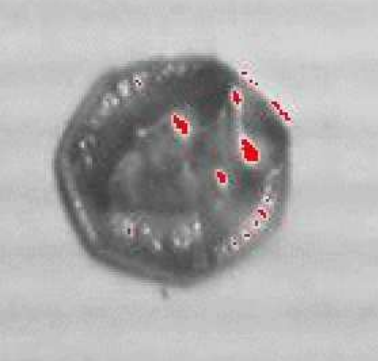
\includegraphics[width=0.3\columnwidth]{specularities.png}
    
    \raggedright
    Solutions: increase ambient lighting by using diffusing panels or lots of point lights, or use smaller aperture, reduce gain and adjust gamma
    
}

\nDefinition{Non-uniform ilumination}{
    Contrast on background enhanced: may cause analysis problems

    \centering
    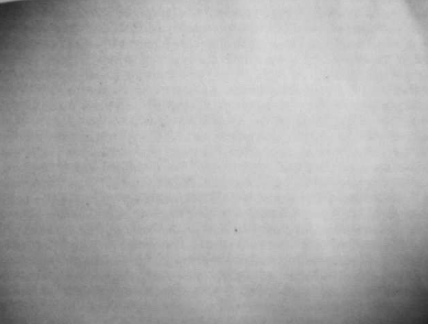
\includegraphics[width=0.3\columnwidth]{non-uniform-ilum.png}

    \raggedright
    Solutions: increase ambient lighting by using diffusing panels or lots of point lights
    
}
\nDefinition{Radial lens distortion}{

    Lenses sometimes slightly distort the image "radially" making accurate measurements hard
    \begin{center}
        \begin{tabular*}{\columnwidth}{m{0.5\columnwidth}m{0.5\columnwidth}}
            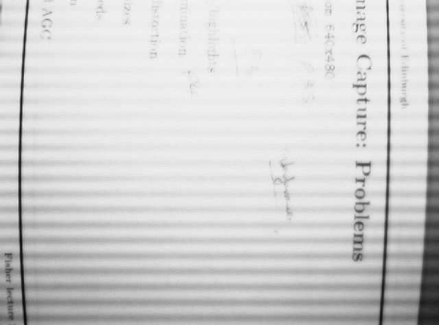
\includegraphics[width=0.35\columnwidth]{radial-lens-distor.png}&
            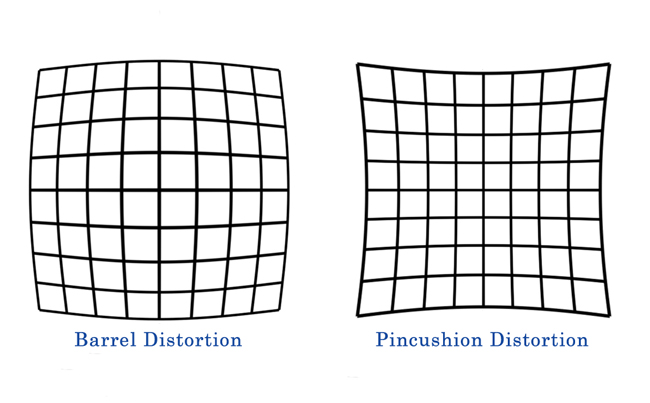
\includegraphics[width=0.35\columnwidth]{lens-distortion-graphic.jpg}
        \end{tabular*}
        \end{center}
    Solutions: more expensive lenses, view from further away
}
\nDefinition{Homography}{
    An invertible linear transformation $\mathbf{P}$ that maps points from one plane to another (think of it as a change of POV)

    \centering
    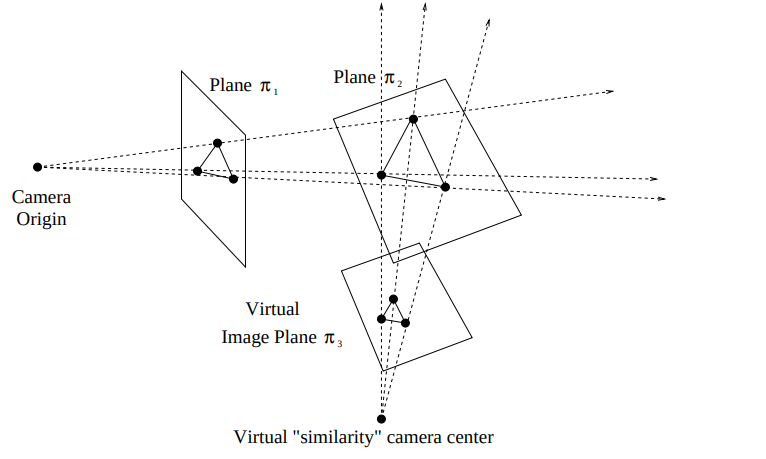
\includegraphics[width=0.8\columnwidth]{homography.png}

    \raggedright

    Given at least 4 corresponding points on each plane defining a POV, we can perform a least-square estimation of $\mathbf{P}$:
    \begin{equation}
        \mathbf{P} = 
        \begin{bmatrix}
            p_{11}&p_{12} &p_{13} \\
            p_{21}&p_{22} &p_{23} \\
            p_{31}&p_{32} &p_{33} 
        \end{bmatrix} 
    \end{equation}

    let $\vec{p} = (p_{11},p_{12} ,p_{13}
        p_{21},p_{22} ,p_{23},
        p_{31},p_{32} ,p_{33})$
        
    let $\mathbf{A}_{i} = 
        \begin{bmatrix}
            0 & 0 & 0 & -u_{i} & -v_{i} & -1 & y_{i}u_{i} & y_{i}v_{i} & y_{i} \\
            u_{i} & v_{i} & 1 & 0 & 0 & 0 & -x_{i}u_{i} & -x_{i}v_{i} & -x_{i} 
        \end{bmatrix}$
    
    construct $\mathbf{A} = 
        \begin{bmatrix}
            A_{1}\\A_{2}\\ \hdots \\ A_{N}
        \end{bmatrix}
    $

    Compute SVD($\mathbf{A}) = \mathbf{UDV'} $
    
    $\vec{p}$ is last column of $\mathbf{V}$ (eigenvector of smallest eigenvalue of $\mathbf{A}$)
    
    Then once we know the homography $\mathbf{P}$, then we can map (u,v) onto (x,y) using:
    \begin{equation}
        \begin{pmatrix}
            \lambda x \\ \lambda y \\ \lambda  
        \end{pmatrix}
        = \mathbf{P}
        \begin{pmatrix}
            u \\ v \\ 1
        \end{pmatrix}
    \end{equation}
    ($\lambda$ representing the fact that this coordinate is in homogenous space)

}

\nSection{Image Segmentation}
\nDefinition{Approaches}{
    Image segmentation is the process of grouping pixels which belong together semantically, i.e. perhaps because they belong to the same object.

    We can segment based on many facts:
    \begin{itemize}
        \item Contrast - objects have different lightness : use thresholding
        \item Change - objects different from background : background models 
        \item Similarity - objects have consistent colours : colour clustering
    \end{itemize}
}

\nDefinition{Thresholding}{
    This method assumes that pixels are separable based on their colour values. We can pick threshold boundaries for each color value and select regions based on 
    regions of pixels which fall in those boundaries.

    \centering
    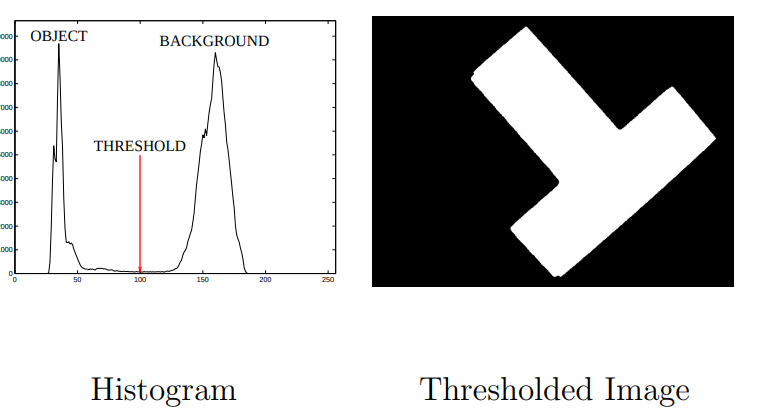
\includegraphics[width=0.8\columnwidth]{thresholding.png}
    \raggedright

    problems:
    \begin{itemize}
        \item Distributions may be broad and have some overlap leading to misclassified pixels
        \item variations in lighting might cause parts of the object to be missing, or shadows to be classified as objects
        \item colour distributions might have more than 2 peaks
    \end{itemize}
}

\nDefinition{Convolutions}{
    General purpose image (and signal) processing function.

    can be used to remve noise, smooth data, or detect features!

    In the case of thresholding, we can use convolutions to smooth the histogram.
    Imagine convolutions as a sliding window, where each point in the original image is replaced with the weighted average of the window at that position with the pixels.

    \centering
    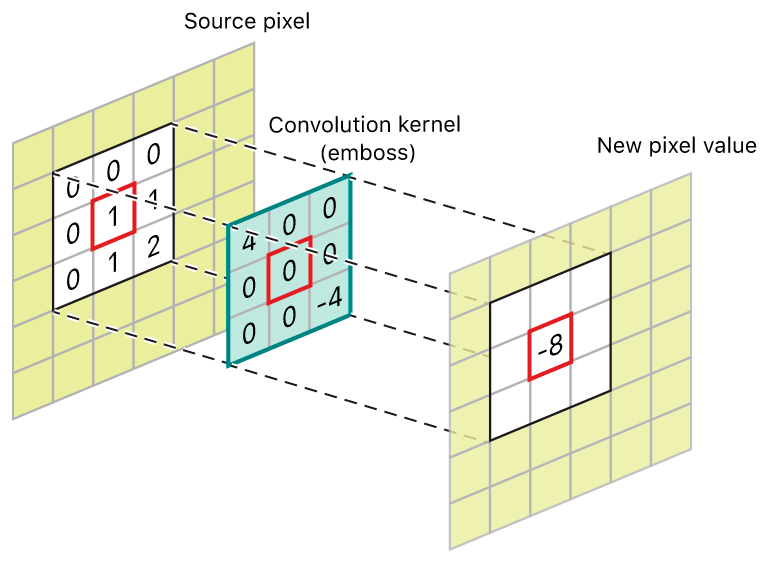
\includegraphics[width=0.8\columnwidth]{convolution.png}

    \raggedright

    Convolution in 1D, with kernel of size (odd) N (even kernels require padding with zeros):
    \begin{equation}
        \textit{Output}(x) = \sum_{i = -\lfloor N/2 \rfloor}^{\lfloor N/2 \rfloor} \textit{weight}(i) * \textit{input}(x - i) 
    \end{equation}

    \centering
    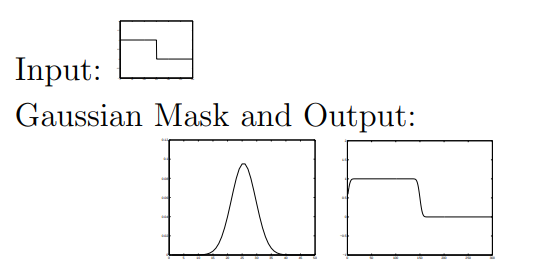
\includegraphics[width=0.5\columnwidth]{convolution_example.png}
    
    \raggedright
    Convolution in 2D, with kernel of size (odd) N:
    \begin{equation}
        \textit{Output}(x) = \sum_{i = -\lfloor N/2 \rfloor}^{\lfloor N/2 \rfloor}\sum_{j = -\lfloor N/2 \rfloor}^{\lfloor N/2 \rfloor} \textit{weight}(i,j) * \textit{input}(x - i,y-j) 
    \end{equation}
}

\nDefinition{Smoothing kernel (2d gaussian)}{
    \centering
    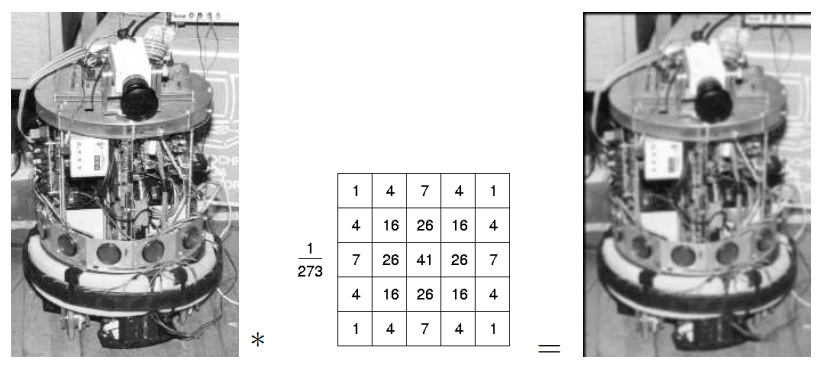
\includegraphics[width=0.9\columnwidth]{smoothing_kernel.png}
}

\nDefinition{Edge Detection kernel}{
    \centering
    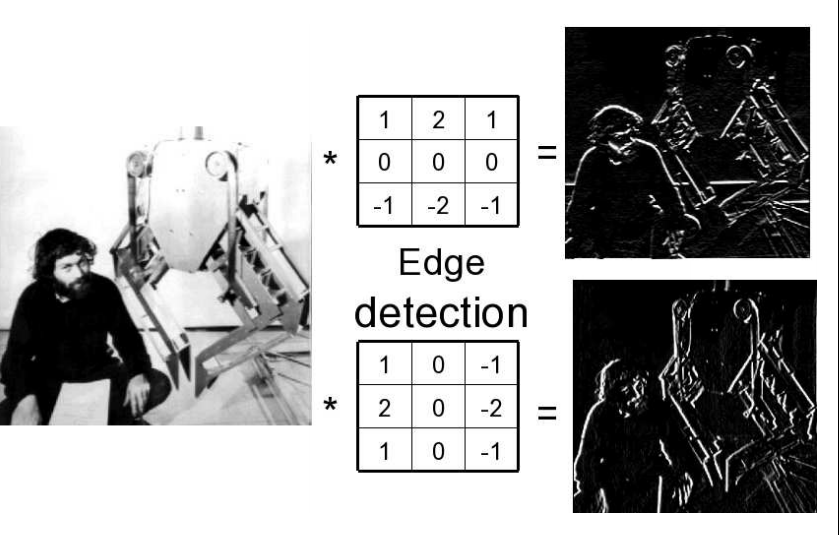
\includegraphics[width=0.9\columnwidth]{edge_detection_kernel.png}

}

\nDefinition{Background removal}{
    If we have 2 images, one with just the background (\textbf{B}) and one with background and foreground (the image \textbf{I}), we can

    \begin{equation}
        N = I - B       
    \end{equation}
    
    This difference will zero-out pixels with identical values to the background, and only leave those values which are different (either positive or negative depending on if the foreground is brighter or darker than the background at each point)

    We can do this for each channel of the image, and perform thresholding on the logical or between all the resulting differential pictures.

    \centering 
    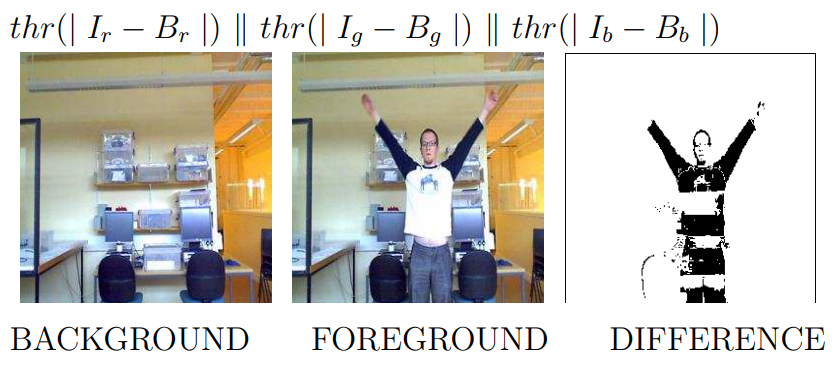
\includegraphics[width=0.7\columnwidth]{bg_differencing.png}

    \raggedright

    we can also use division instead of substraction to achieve a similar effect:
    \begin{equation}
        N = I / B
    \end{equation}

    This in effect removes the effects of illumination since:

    \begin{equation}
        \textit{background}(i,j) = \textit{illumination}(i,j) \cdot \textit{bg\_reflectance}(i,j)
    \end{equation}
    \begin{equation}
        \textit{object}(i,j) = \textit{illumination}(i,j) \cdot \textit{obj\_reflectance}(i,j)
    \end{equation}

    The pixels with a value of 1 are going to be the background, pixels with value $>$ 1 are lighter objects and pixels with values $<$ 1 are darker objects (than the background)

    In both of these techniques, we might need to use an operator such as the \textbf{open} operator to remove noise artifacts (with values which are just around the values which signify background pixels but not quite)

    Neither will work well when the background in I and B varies wildly.

}

\nDefinition{RGB Normalisation}{
    differences in lighting can be dealt with by normalising the RGB values of the image:

    \begin{equation}
        (r',g',b') = (\frac{r}{r+g+b},\frac{g}{r+g+b},\frac{b}{r+g+b})
    \end{equation}

    since multiplying all values r,g,b in the original space by a constant, changes the brightness of the color, we remove this effect thanks to the equation above,
    mapping all different brightness values of the same colour to one value.

    \centering
    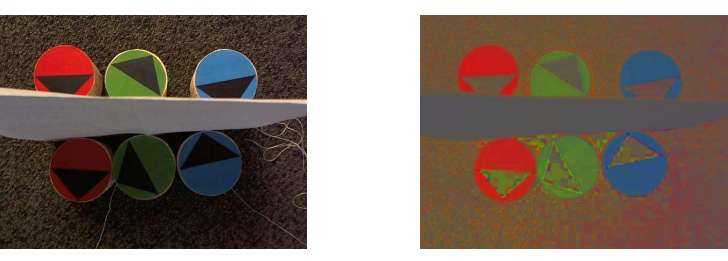
\includegraphics[width=0.5\columnwidth]{rgb_normalisation}
}

\nDefinition{Mean Shift Segmentation}{
    We can segment the image by performing clustering on the pixels by their color values (or any attributes for that reason)!

    The algorithm works as follows:

    \begin{enumerate}
        \item create a feature space over the attributes chosen to represent each pixel (for example for a grayscale this could be a 1d intensity axis)
            \newline 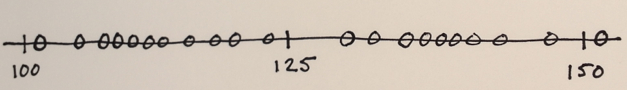
\includegraphics[width=0.7\columnwidth]{msc_0.png}
        \item distribute a number of "search windows" or kernels over the space 
            \newline 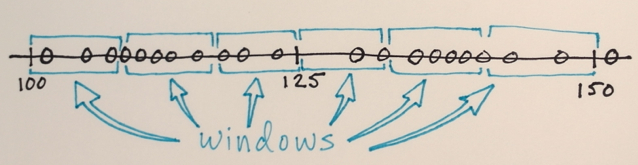
\includegraphics[width=0.7\columnwidth]{msc_1.png}
        \item calculate each window's mean 
        \item shift the center of each window to its mean 
            \newline 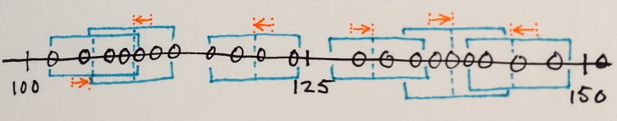
\includegraphics[width=0.7\columnwidth]{msc_3.png} 
        \item repeat steps 3-4 until convergence 
            \newline 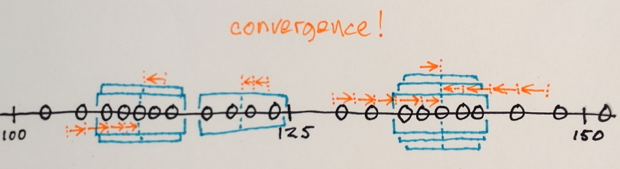
\includegraphics[width=0.7\columnwidth]{msc_4.png}
        \item merge windows ending up in close-enough locations, and call these the clusters
        \item cluster each pixel according to which cluster its original window ended up at 
            \newline 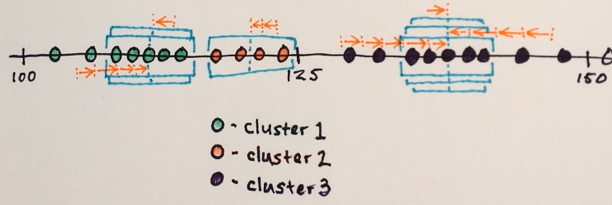
\includegraphics[width=0.7\columnwidth]{msc_5.png}
    \end{enumerate}

    the feature space can contain any number of dimensions, and so we could include spatial, color, texture-data, and so on. This is a very versatile algorithm.
    It is application-independent, model-free (does not assume any shape of clusters),
    only requires a single parameter (window size h) which affects the scale of the clustering
    It is robust to outliers and finds a variable number of modes given the same h.

    The output is heavilly dependent on the window size h, however. And the selection of h is not trivial. The whole algorithm is rather expensive and does not scale well with the dimension of the feature space.
    }

\end{document}
